\documentclass[a4paper, 12pt]{article}

%%% Работа с русским языком
\usepackage{cmap}					% поиск в PDF
\usepackage{mathtext} 				% русские буквы в формулах
\usepackage[T2A]{fontenc}			% кодировка
\usepackage[utf8]{inputenc}			% кодировка исходного текста
\usepackage[russian]{babel}	% локализация и переносы

%%% Дополнительная работа с математикой
\usepackage{amsmath,amsfonts,amssymb,amsthm,mathtools} % AMS
\usepackage{icomma} % "Умная" запятая: $0,2$ --- число, $0, 2$ --- перечисление

%% Номера формул
%\mathtoolsset{showonlyrefs=true} % Показывать номера только у тех формул, на которые есть \eqref{} в тексте.

%% Шрифты
\usepackage{euscript}	 % Шрифт Евклид
\usepackage{mathrsfs} % Красивый матшрифт

%% Поля
\usepackage[left=2cm,right=2cm,top=2cm,bottom=2cm,bindingoffset=0cm]{geometry}

%% Русские списки
\usepackage{enumitem}
\makeatletter
\AddEnumerateCounter{\asbuk}{\russian@alph}{щ}
\makeatother

%%% Работа с картинками
\usepackage{graphicx}  % Для вставки рисунков
\graphicspath{{images/}{images2/}}  % папки с картинками
\setlength\fboxsep{3pt} % Отступ рамки \fbox{} от рисунка
\setlength\fboxrule{1pt} % Толщина линий рамки \fbox{}
\usepackage{wrapfig} % Обтекание рисунков и таблиц текстом

%%% Работа с таблицами
\usepackage{array,tabularx,tabulary,booktabs} % Дополнительная работа с таблицами
\usepackage{longtable}  % Длинные таблицы
\usepackage{multirow} % Слияние строк в таблице

%% Красная строка
\setlength{\parindent}{2em}

%% Интервалы
\linespread{1}
\usepackage{multirow}

%% TikZ
\usepackage{tikz}
\usetikzlibrary{graphs,graphs.standard}

%% Верхний колонтитул
\usepackage{fancyhdr}
\pagestyle{fancy}

%% Перенос знаков в формулах (по Львовскому)
\newcommand*{\hm}[1]{#1\nobreak\discretionary{}
	{\hbox{$\mathsurround=0pt #1$}}{}}

%% Мои дополнения
\usepackage{float} %Добавляет возможность работы с командой [H] которая улучшает расположение на странице
\usepackage{gensymb} %Красивые градусы
\usepackage{graphicx}               % Импорт изображений
\usepackage{caption} % Пакет для подписей к рисункам, в частности, для работы caption*

% подключаем hyperref (для ссылок внутри  pdf)
\usepackage[unicode, pdftex]{hyperref}

%%% Теоремы
\theoremstyle{plain}                    % Это стиль по умолчанию, его можно не переопределять.
\renewcommand\qedsymbol{$\blacksquare$} % переопределение символа завершения доказательства

\newtheorem{theorem}{Теорема}[section] % Теорема (счетчик по секиям)
\newtheorem{proposition}{Утверждение}[section] % Утверждение (счетчик по секиям)
\newtheorem{definition}{Определение}[section] % Определение (счетчик по секиям)
\newtheorem{corollary}{Следствие}[theorem] % Следстиве (счетчик по теоремам)
\newtheorem{problem}{Задача}[section] % Задача (счетчик по секиям)
\newtheorem*{remark}{Примечание} % Примечание (можно переопределить, как Замечание)
\newtheorem{lemma}{Лемма}[section] % Лемма (счетчик по секиям)

\begin{document}
    \newcommand{\HRule}{\rule{\linewidth}{0.7mm}} % Defines a new command for the horizontal lines, change thickness here
	
	\begin{center}
		\large\textbf{Московский Физико-Технический Институт}\\ % Name of your university/college
		\large\textbf{(государственный университет)}
	
		\vfill
		
		\Large Лабораторная работа по курсу общей физики № *labnum*\\[0.5cm] % Preambule of your document title
		
		
		\HRule
		\\[0.4cm]
		{ \huge \bfseries *name of your labwork*}% Title of your document
		\\[0.4cm] 
		\HRule
		\\[0.5cm]
		
		\ \\
	\textbf{\large Автор:} \\	
	\large *your name* *groupname*\\ % Your name and something more, your group num for example
		\vfill
		\hspace*{-0.8 cm}
\includegraphics[width=100 pt]{frkt_logo}\\ % logo of your  company/university/college
		\large Долгопрудный, 2021 % location and year
	\end{center}

\newpage
\setcounter{page}{2}
\fancyfoot[c]{\thepage}
\fancyhead[L] {Работа № *labnum*} % some information in page header
\fancyhead[R]{}

    \paragraph*{Цель работы:} Исследуется электронный парамагнитный резонанс в молекуле ДФПГ, определяется $g$-фактор электрона, измеряется ширина ЭПР.                                                                              

    \section*{Теоретическое введение}
        Энергетический уровень электрона в присутствии магнитного поля с индукцией $B$ расщепляется на подуровня, расстояние между которыми равно 
        \begin{equation}
            \label{eq:dE}
            \Delta E = E_2 - E_1 = 2\mu B.
        \end{equation}
        Здесь $\mu$ -- абсолютная величина проекции магнитного момента на направление поля.
        
        Между этими двумя уровнями возможны переходы. Эти переходы могут возбуждаться внешним высокочастотным электромагнитным полем, если оно имеет нужную частоту и нужное направление.
        
        Резонансное значение частоты определяется из очевидной формулы:
        \begin{equation}
            \label{eq:resonans_omega}
            \hbar \omega_0 = \Delta E.
        \end{equation}

        При переходе с нижнего на верхний уровень энергии электрон поглощает квант электромагнитной энергии, а при обратном переходе такой же квант излучается. Возбуждение электронных резонансных переходов электромагнитным полем, имеющим частоту, определяемую формулой~(\ref{eq:resonans_omega}), носит название электронного парамагнитного резонанса (ЭПР).
        
        В настоящей работе необходимо получить сигнал ЭПР на кристаллическом дифенилпикрилгидразиле (ДФПГ) и определить значение $g$-фактора для электрона. Как известно, связь между магнитным моментом $\mu$ электрона и его механическим моментом $\mathbf{M}$ выражается через гиромагнитное отношение $\gamma$ с помощью формулы
        \begin{equation}
            \label{eq:gyromagnit}
            \mu = \gamma M.
        \end{equation}
        
        Если магнитный момент частицы, измеренный в магнитонах Бора, а механический - в $\hbar$, то их связь можно записать через $g$-фактор:
        \begin{equation}
            \label{eq:def_g}
            \frac{\mu}{\mu_\text{Б}} = \frac{g M}{\hbar} 
        \end{equation}

        Используя соотношения (\ref{eq:dE})-(\ref{eq:def_g}), нетрудно получить выражение для $g$-фактора через определяемые экспериментально величины:
        \begin{equation}
            \label{eq:g_is}
            \tag{$\star$}
            g = \frac{\hbar \omega_0}{\mu_\text{Б} B}.
        \end{equation}

    \newpage
    
    \section{Экспериментальная установка}
    
    Образец (порошок ДФПГ) в стеклянной ампуле помещяется внутрь катушкииндуктивнсоти входящей в состав колебательного контура. Входящий в состав контура конденсатор состоит из двух платсин, разделенных воздушным зазором, одна из пластин может перемещаться поворотом штока. Колебания в контуре возбуждаются антенной, соединённой с генератором частоты (ВЧ) Г4-116. Амплитуда колебаний поля в катушке индуктивности измеряется по наводимой в петле связи ЭДС индукции. Высокочастотные колебания ЭДС индукции в приёмном контуре детектируются диодом, измеряемая при помощи осциллографа низкочастотная огибающая этого сигнала пропорциональна квадрату амплитуды колебаний поля в катушке.
    \begin{figure}[h!]
        \centering
            \caption{Схема установки.}
            \label{fig:equip}
            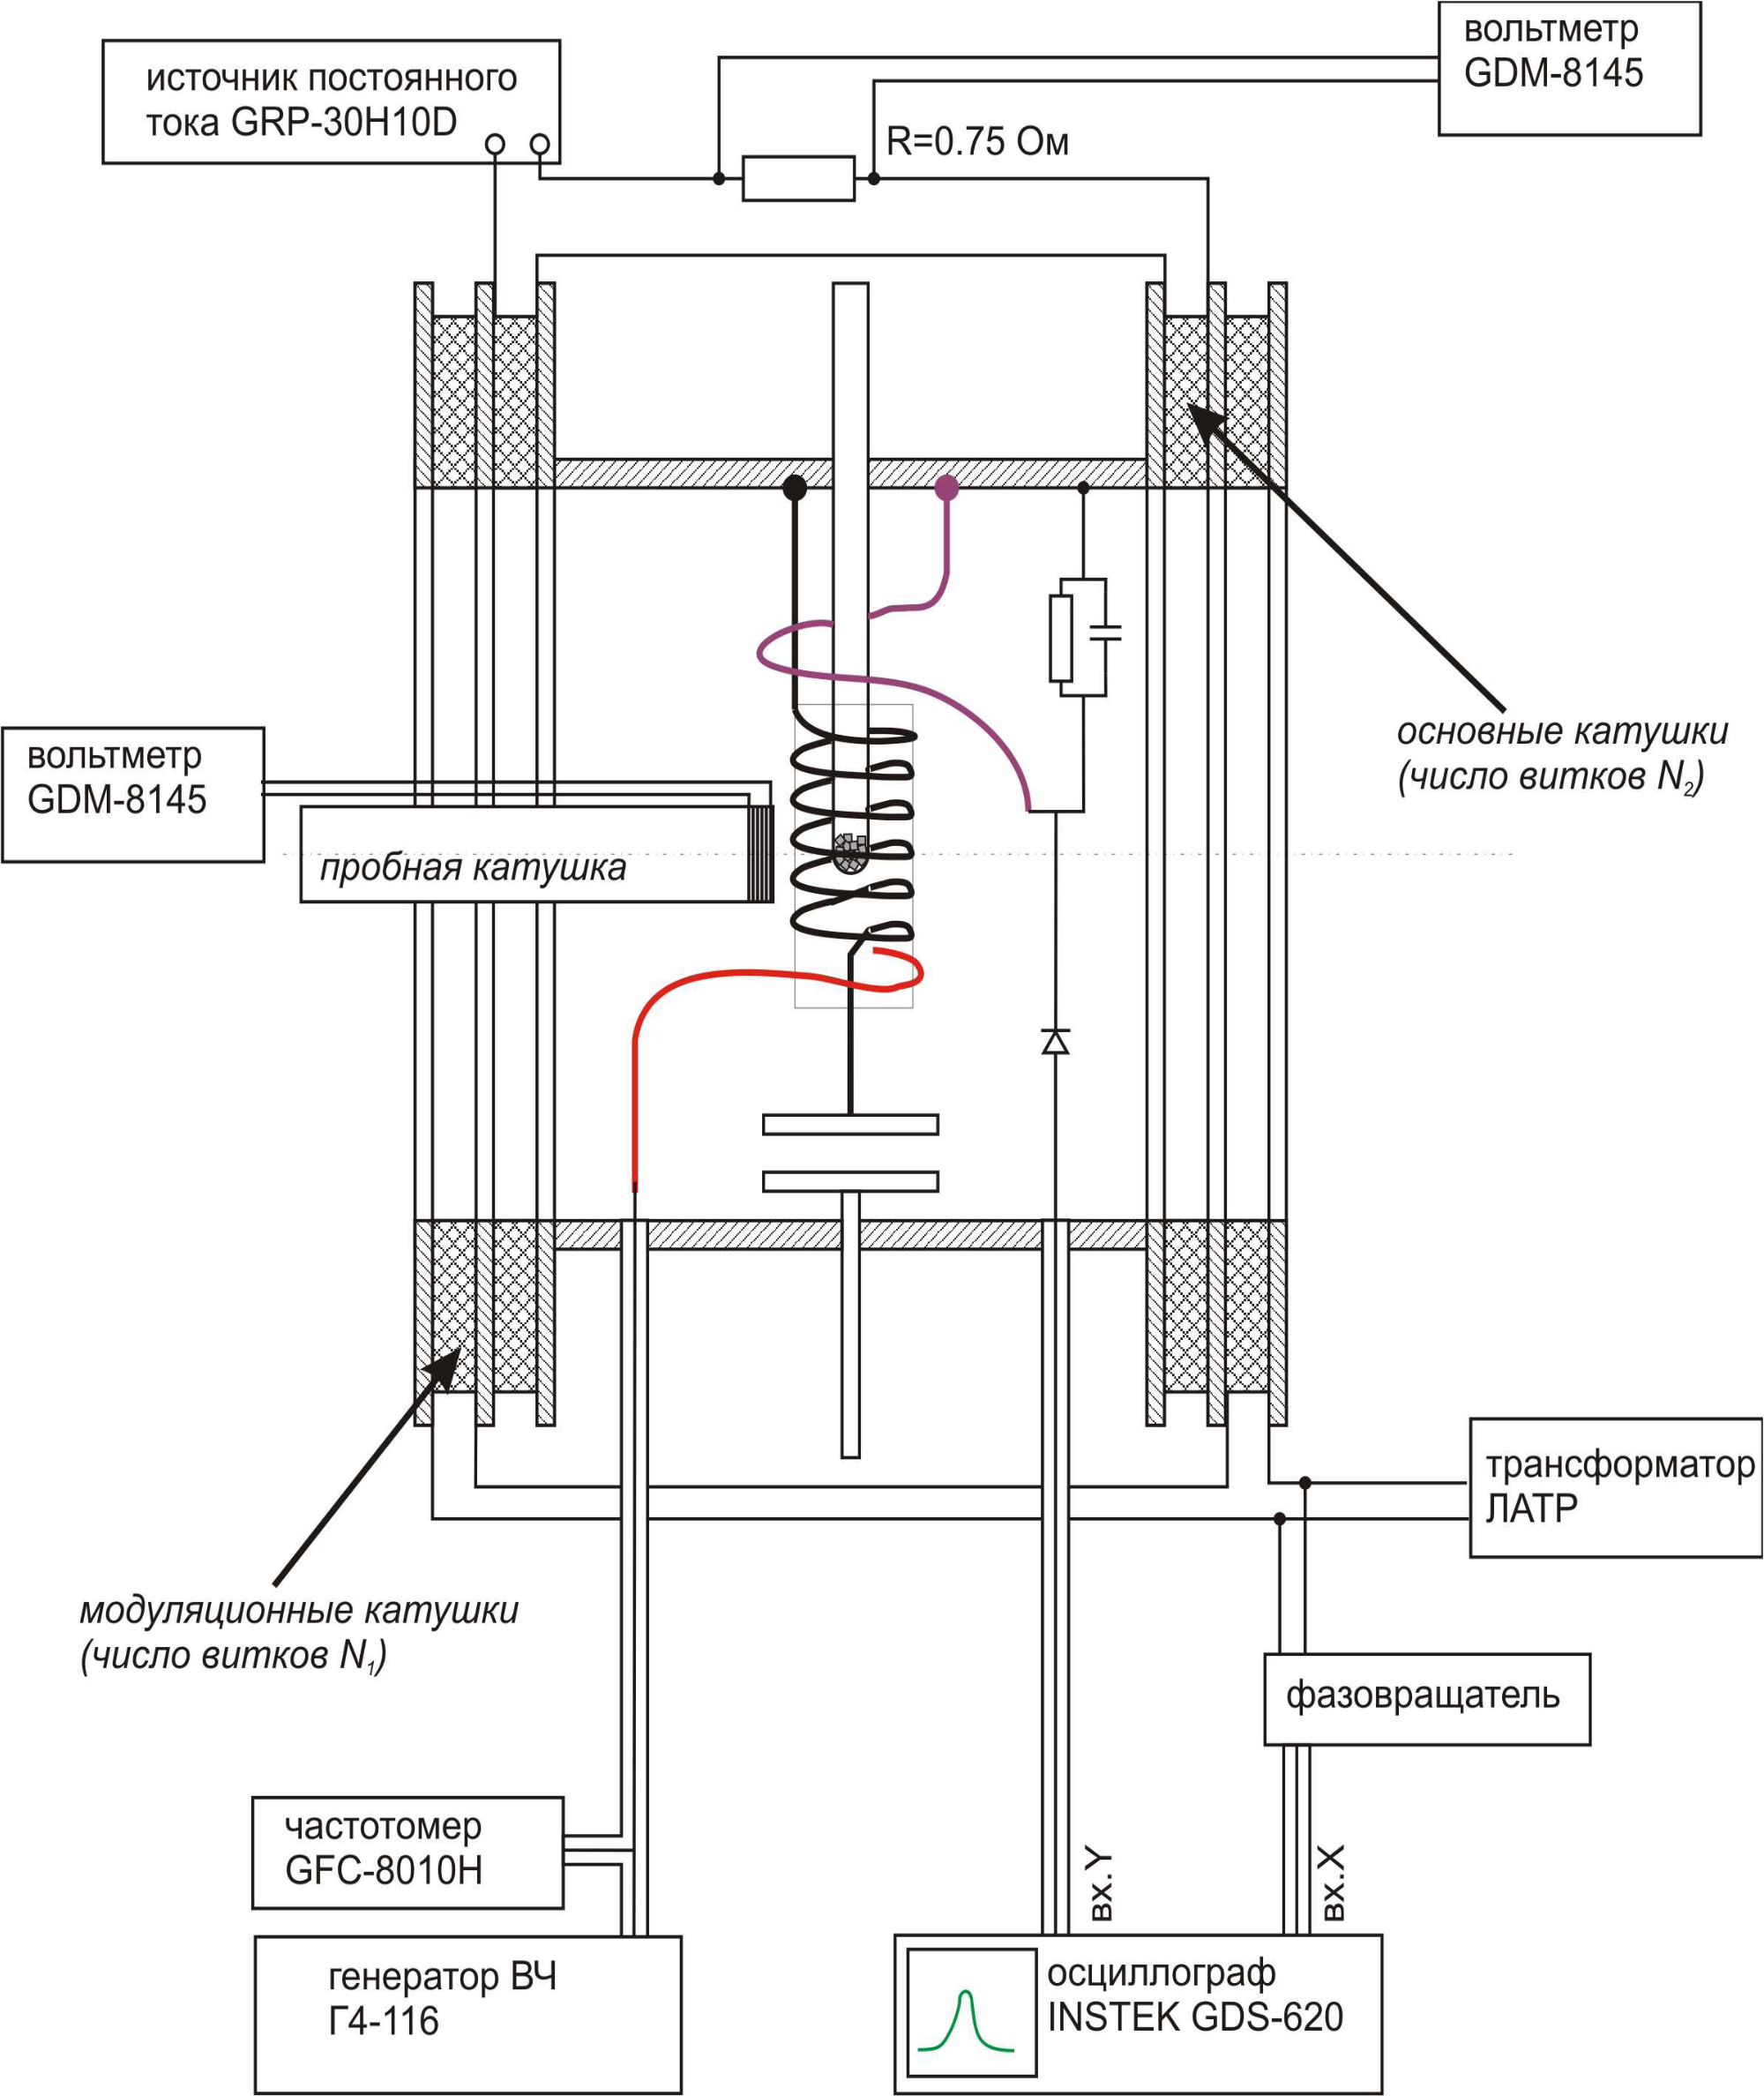
\includegraphics[scale=0.17]{equip.png}
    \end{figure}
    
    Постоянной магнитное поле создаётся пропусканием тока от источника постоянного тока через основные катушки. При этом при помощи вольтметра измеряется падение напряжения на резисторе в цепи основных катушек. Переменное поле небольшой амплитуды создаётся подачей на модуляционные катушки напряжения с регулируемого трансформатора ЛАТР. Для измерения амплитуды колебаний переменного поля используется пробная катушка известной геометрии, подключенная к вольтметру.

    \section*{Ход работы}
    
    Запишем параметры катушек в  Таблицу \ref{table:coils}:
    
    \begin{table}[h]
    \centering
        \begin{tabular}{|l|l|l|}
        \hline
        \textbf{Катушка} & $N$ & $D$, см \\ \hline \hline
        Основная         & 6700         & $25\pm1$             \\ \hline
        Модуляционная    & 5000         & $30\pm1$             \\ \hline
        Пробная          & 45           & $1.52\pm0.01$             \\ \hline
        \end{tabular}
        \caption{Параметры катушек.}
        \label{table:coils}
    \end{table}
    
    \subsection*{Резонанс}
    
    
    Настроим генератор на частоту колебательного конутра. Получаем резонансную частоту:
    \begin{equation*}
        f_0 = (164 \pm 1) \ \text{Мгц}.
    \end{equation*}

    Подберем величину постоянного магнитного поля в катушках так, чтобы наблюдался сигнал резонанского поглощения. Для этого подадим на катушки достаточное напряжение.
    
    Для более точной настройки и определения ширины линии резонасного поглощения будем наблюдать сигнал в $XY$-режиме. Запишем значение напряжения на резисторе в цепи основных катушек:
    \begin{equation*}
        U_0 = (130 \pm 1) \ \text{мВ}.
    \end{equation*}
    
    \subsection*{Ширина линии поглощения}

    Определим ширину линии ЭПР (полуширина на на полувысоте линии резонасного поглощения):
    \begin{equation*}
        \Delta B = \frac{A_{1/2}}{A_{\text{полн}}}B_\text{мод},
    \end{equation*}
    где $A_\text{полн}$ -- полный размах модулирующего поля, $A_{1/2}$ -- ширина кривой на полувысоте, $B_\text{мод}$ -- амплитуда модулирующего поля.
    \begin{equation*}
        \begin{gathered}
            A_\text{полн} = (10 \pm 0.2 ) \ \text{дел}, \ A_{1/2} = (3 \pm 0.2) \ \text{дел} \\
            B_\text{мод} = \sqrt{2} \frac{2\varepsilon}{\pi^2d^2N\nu} = 0.75\pm 0.05 \text{мТл},
        \end{gathered}
    \end{equation*}
    где $\varepsilon$ -- ЭДС индукции при внесении пробной катушки, $N$ -- число витков катушки, $d$ -- диаметр катушки, $\nu$ -- частота модулирующего напряжения (50 Гц).
    
    Имеем:
    \[\boxed{\Delta B = (0.22 \pm 0.02) \ \text{мТл}}.\]
    
    \subsection*{Калибровка основной катушки}
    
    Определим связь между падением напряжения на резисторе в цепи основных катушек и магнитным полем в центре магнита. Поле в центре будем измерять, поднося пробную катушку. 
    Результаты занесем в Таблицу \ref{table:field}: 
    
    \begin{table}[h]
    \centering
        \begin{tabular}{|c|c|c|c|c|c|}
        \hline
        $V_R$, мВ              & 3.52 & 5.35 & 7.14 & 8.90 & 10.53 \\ \hline
        $V$, мВ  & 0.44 & 0.65 & 0.85 & 1.07 & 1.255 \\ \hline
        \end{tabular}
    \caption{Калибровочные измерения.}
    \label{table:field}
    \end{table}
    
    По полученным данным построим калибровочный график (считаем, что он проходит через начало координат)
    и определим коэффициент наклона.

    \begin{figure}
        \centering
        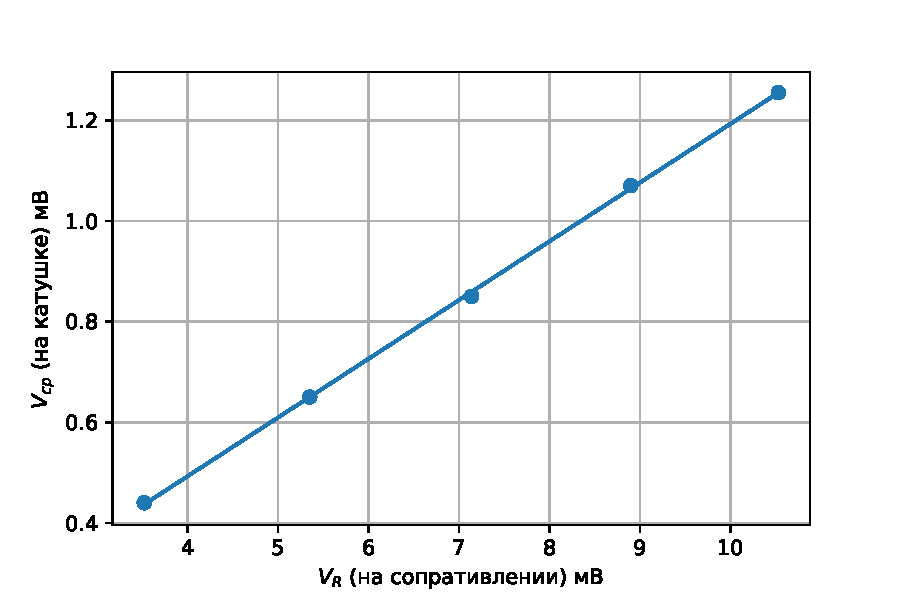
\includegraphics[scale=1]{calibration.pdf}
        \caption{Калибровочный график}
        \label{fig:calibration}
    \end{figure}

    Значение коэффициента наклона 

    \[ k = (11.7 \pm 0.1) \cdot 10^{-2} \]

    Для упрощения расчетов будем считать, что $k \approx 0.12$.


    Рассчитав поле, создаваемое основными катушками,
    
    \begin{equation*}
        B_0 = \frac{4 k U_0}{2\pi\nu N \pi d^2} = (6.1 \pm 0.1) \text{мТл}.
    \end{equation*}
    
    Найдем $g$-фактор электрона:
    
    \begin{equation*}
        g = \frac{hf_0}{\mu_BB_0} = 1.9 \pm 0.1
    \end{equation*}
    

    \section*{Вывод}
	
    В данной работе был исследован ЭПР в молекуле ДФПГ, определяется $g$-фактор электрона $g = 1.9 \pm 0.1$, а также измерена ширина линий ЭПР $\Delta B = 0.22 \pm 0.2~\text{мТл}$. 
	
    Измеренный $g$-фактор электрона совпадает с табличным значением для свободного электрона: $g = 2.0$. Это обусловлено тем, что ПР происходит на неспаренных электронах так же, как на свободных.
	

\end{document}
